\documentclass[a4paper]{article}
\hoffset=-0.55in
\textwidth=5.9in
\voffset=-0.5in
\textheight=10in
\usepackage{graphicx}
\usepackage{caption}
\usepackage{hyperref}
\begin{document}
\addtolength{\voffset}{-0.5in}
\pagestyle{empty}
\setlength\parskip{5pt}
\title{Data scientist assignment}
\author{Sam Blake}
\maketitle
For this assignment I was pointed towards a US Department of Transportation dataset of every domestic flight in the USA between 1987 and the present, and given additional datasets containing the names of the airline carriers and the locations of the airports. I was given the brief: \\
\textit{``imagine you are working as data scientist at one of the Airline companies and you were given the problem of comparing and optimizing performance for that company''}\\
and a week to complete the task. To this end, I looked at the number of cancellations and average delays for all airlines in 2015 -- and the effect on these of geography and seasonal variation -- and built a classifier for predicting which flights would be cancelled. In this document I'll summarise my investigation and findings, but I have also put the IPython notebooks, in which I performed all the analysis, on my github account at \url{https://github.com/sfblake/Flights_Project}.

\section*{Data exploration}

\subsection*{The data}
Each year there are millions of domestic flights within the USA, and for each flight the Department of Transportation records over 100 variables. Stretching back to 1987 this is a lot of rows of data (a single year, in .csv format, comes in at over a GB) so, due to the constraints of time and computing power, I limited my analysis to the most recent year's worth of data: 2015 (as the data will be used to assess carrier performance and predict future behaviour, taking the most recent year seems sensible). In 2015 there are over \textbf{5.8 million flights}, shared between \textbf{14 carriers} (i.e. airlines) and \textbf{322 airports}.

For each flight the dataset contains mainly information the airlines would know beforehand: the date and time of each flight, origin and destination airports etc. However the dataset also makes note of whether a flight was cancelled or diverted, or otherwise how long it was delayed by. These all cost the airlines money: although (unlike the EU) the USA has no federal regulations for paying out to customers on delays and cancellations,  most airlines will cover food and accomodation or offer a refund for a `substantial' (definitions vary) delay or cancellation.\footnotemark[1]\footnotetext[1]{\url{http://www.huffingtonpost.com/smartertravel/a-guide-to-air-passenger_b_4017963.html}} These costs are estimated at \textbf{${\sim}$\$70 per minute delayed} and \textbf{${\sim}$\$5,000 - \$11,000 per cancellation} (depending on the size of plane) totalling to around \textbf{\$22 billion} a year across all airlines in the USA\footnotemark[2]\footnotetext[2]{\url{https://books.google.co.uk/books?id=4yOeWfX5gekC&pg=PA16}}. Therefore evaluating airline performance on delays and cancellations -- and predicting which flights are most likely to be affected -- is of great value to the business.

\subsection*{Evaluating airline performance}
To determine how well each airline performs on delays and cancellations in 2015, I calculated, for each airline, the {\bf mean flight delay} and the {\bf percentage of flights which were cancelled}. Many flights in fact leave before their departure time and so have a `negative' departure delay, however I treated these as having a departure of 0: there is no `profit' gained from leaving early equivalent to the costs of being delayed -- these early flights are simply on time. By taking the previously quoted costs for delays and cancellations (and assuming a cost per cancellation of \$8,000, in the middle of the quoted range) I also calculated a rough estimate of the total cost to the airline of delays and cancellations. As the airlines each run a different number of flights however, comparing these numbers between airlines would not give a fair comparison -- instead I divided the total cost by the number of flights to get an estimate of the {\bf cost per flight due to delays and cancellations}.

\begin{figure}[h]
\centering
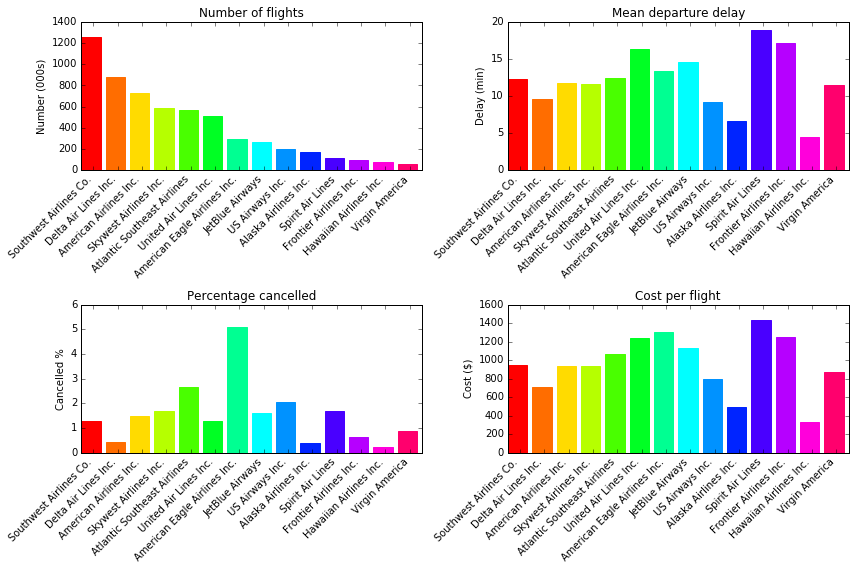
\includegraphics[width=\textwidth]{../figures/exploration/cost_carrier.png}
\caption{Delay and cancellation performace of airlines in 2015}
\label{costbycarrier}
\end{figure}

Figure \ref{costbycarrier} shows the total number of flights, mean flight delay, percentage cancellation and cost per flight for each airline in 2015. The number of flights varies from 1.2 million (Southwest) to $<$100 thousand (Virgin America) but there is no clear economy of scale in play -- the delays and cancellations have no dependence on airline size. Indeed two of the smallest airlines -- Alaska and Hawaiian -- have the lowest mean delays ($<$5 minutes) and costs per flight, but the two airlines between them in size -- Spirit and Frontier -- have some of the highest ($>$15 minutes). American Eagle also stands out in the Figure as by far the most cancellation-happy airline, with 1 in 20 of its flights being cancelled. So why our Alaska and Hawaiian having fewer delays and cancellations? The clue may lie in their names: both are serving specific -- and peripheral -- parts of the USA.

\subsection*{Geographical variation}

To look at the exact positions of the airports I used the latitude and longitude coordinates given in the ancillary file; unfortunately some airports were lacking from this dataset, so I automated the look up of these using the Google Maps api.\footnotemark[3]\footnotetext[3]{\url{http://py-googlemaps.sourceforge.net/}} Figure \ref{airportscarrier} shows the most used airports in 2015 both in total and by carrier: the size of each airport on the map indicates the total number of flights departing in the year, normalised by the total number of flights run by the airline. 

The `Total' map looks as one may expect, with the large urban centres having the busiest airports, but the individual airline maps show a lot more variation. The bigger airlines fall into two categories: those, such as Southwest and Skywest, which run a point-to-point network, in which flights are run between most airports; and those, such as Delta and American Airlines, which run a hub-and-spoke network, where most flights are to or from a central hub (Atlanta for Delta and Dallas for American Airlines). The smaller airlines tend to focus on a particular region of the USA, such as the Midwest for American Eagle and the East Coast and Puerto Rico for JetBlue. As expected Alaska airlines services mainly Alaska (and the Pacific North West) and Hawaiian Hawaii. Interestingly the two poorest performing small airlines in terms of delays, Spirit Air and Frontier, do not run a regional service but instead a national point-to-point and hub-and-spoke network respectively. There may therefore be an economy of size after all: smaller airlines whose resources are spread across a national -- rather than regional -- network have longer mean delays.

\begin{figure}[h]
\centering
\hbox{\hspace{-0.7in}
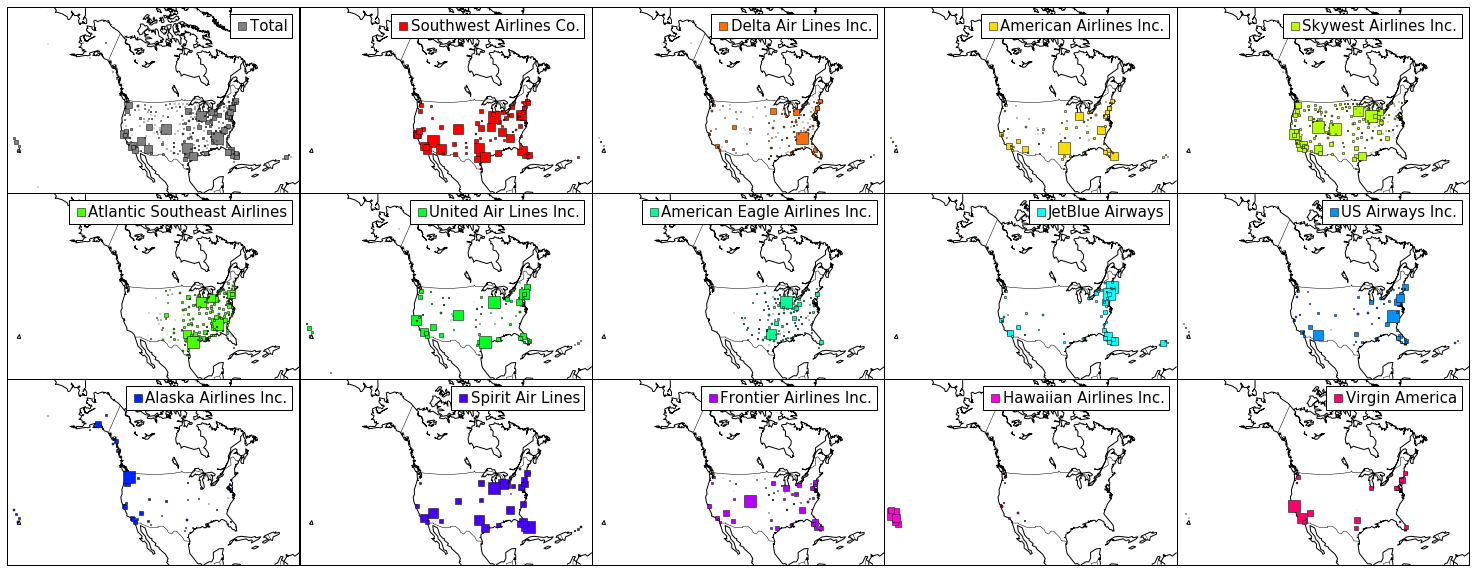
\includegraphics[width=1.2\textwidth]{../figures/exploration/airports_carrier.png}}
\caption{Most used airports by airline in 2015}
\label{airportscarrier}
\end{figure}

In order to see the geographical variation of delays and cancellations, I calculated the mean delay and percentage cancelled for each individual airport; these are shown in Figure \ref{costairports}. The size of each airport still indicates its number of departures in the year (though scaled by the square root in this case so that more airports can be seen), but the colour now represents the respective variable. Considering first the delays, these are shortest for airports in the North West and Hawaii -- the exact regions served by the two best performing airlines, Alaska and Hawaiian. This suggests that the reason for their low mean delay times may be geographical. Comparing these regions with those of the longest mean delays -- in the North East on the Atlantic seaboard and around the Great Lakes, and in the South East in Florida and along the Gulf of Mexico -- the obvious difference is one of climate: the North East is often hit by snow storms in winter, and the South East by tropical storms in summer; the North West and Hawaii do not have such extreme weather events. The mean departure delay map therefore looks much like a combination of the maps of yearly snowfall\footnotemark[4]\footnotetext[4]{\url{https://commons.wikimedia.org/wiki/File:United_states_average_annual_snowfall.jpg}} and hurricane activity\footnotemark[5]\footnotetext[5]{\url{http://maps.redcross.org/website/Maps/Images/NationalLevel/hurricane.gif}} in the USA. The cancellation map also shows a similar regional dependence, although a higher proportion of flights appear to be cancelled due to snow in the North East than tropical storms in the South East. The Midwest and Texas also have a higer percentage cancelled, and this is where American Eagle -- which cancelled by far the highest proportion of flights -- mainly operates. Although away from the winter storms and tropical storms of the East Coast, this region is sometimes known as `Tornado Alley'\footnotemark[6]\footnotetext[6]{\url{http://strangesounds.org/wp-content/uploads/2014/04/tornado-risk-map.jpg}} due to the high winds that sometimes occur, so again extreme weather phenomena seem to result in more cancellations.

\begin{figure}[h]
\centering
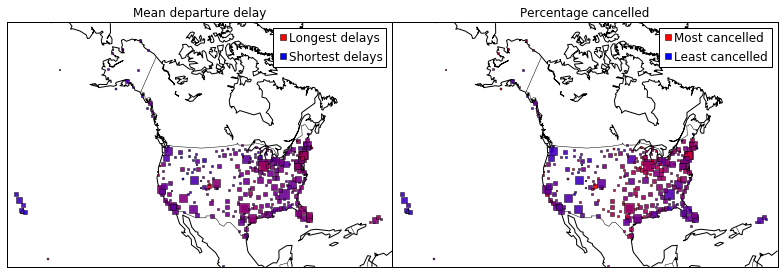
\includegraphics[width=1\textwidth]{../figures/exploration/cost_airports.png}
\caption{Delay and cancellation performace of airports in 2015}
\label{costairports}
\end{figure}

To get a measure of each airline's performance independent of the regions it serviced, I looked at their performance compared to their airports' means: that is, for each airport used, I calculated how much longer (or shorter) the airline's mean delay was than the average; and whether the airline was cancelling a higher (or smaller) percentage of flights. This means each airline's performance can be judged against the other airlines that it shares airports with. The top two panels of Figure \ref{normalisedcostbycarrier} shows these values for each airline: the two small airlines running a national service, Spirit and Frontier, will have considerably longer delays at an airport than other airlines; while American Eagle is indeed more likely to cancel a flight than its competitors. These airport-normalised delays and cancellations can be combined, as before, to obtain a cost per flight: the bottom left panel of Figure \ref{normalisedcostbycarrier} shows each airline's performance in cost compared to the airport mean; the bottom right panel shows the actual cost for each airline (the same as the bottom right panel of Figure \ref{costbycarrier}), with a black line indicating what each airline's cost would be if all its flights had the average delay and average likelihood of cancellation of their departure airport. This illustrates that hub-and-spoke networks have fewer delays and cancellations than point-to-point networks: Delta and American Airlines -- both hub-and-spoke -- perform better than average, while Southwest, Skywest and Atlantic Southeast -- all point-to-point -- perform close to, or just below average. For smaller airlines, those serving regions of the USA, rather than its entirety, perform better: although Alaska and Hawaiian both have favourable geography -- their black lines of cost per flight given airport average are below all other airlines' -- they nevertheless outperform their airports' average; Frontier and Spirit -- both operating flights nationwide -- perform considerably worse than their airports' average.

\begin{figure}[h]
\centering
\hbox{\hspace{-0.5in}
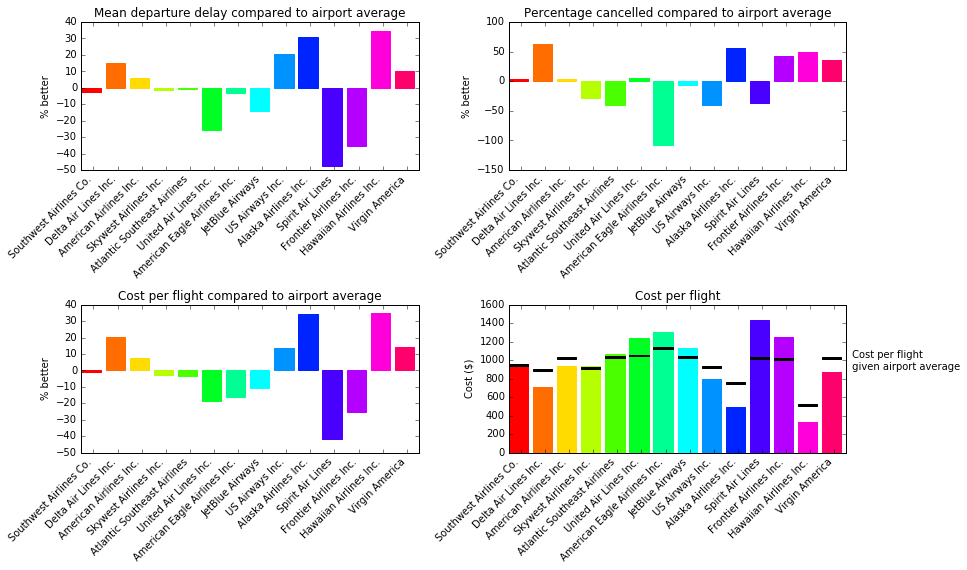
\includegraphics[width=1.2\textwidth]{../figures/exploration/normalised_cost_carrier.png}}
\caption{Delay and cancellation performace of airlines in 2015, normalised by airport}
\label{normalisedcostbycarrier}
\end{figure}

\subsection*{Temporal variation}
In the previous section I found that geography (or specifically, it seems, weather) has a large effect on delays and cancellations, and that the airline operating the flight also contributes. In the Department of Transportation dataset the date and time of each flight is also specified, so next I investigated whether this had an effect on cancellations. Firstly, to see what external events have an influence on the dataset, I looked at the variation in the daily number of flights over 2015.

\begin{figure}[h]
\centering
\hbox{\hspace{-0.5in}
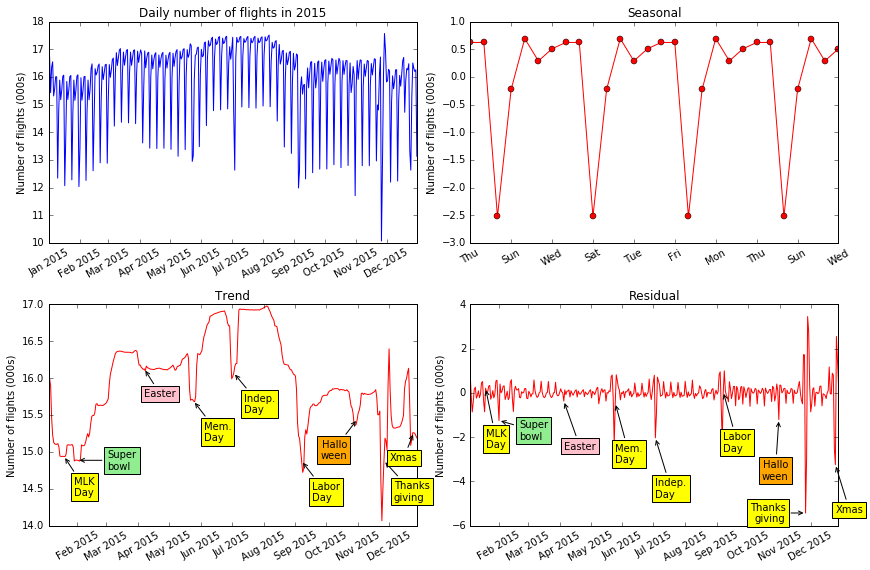
\includegraphics[width=1.1\textwidth]{../figures/exploration/num_flights_year.png}}
\caption{Variation in the daily number of flights through 2015}
\label{numflightsyear}
\end{figure}

The top left panel of Figure \ref{numflightsyear} shows the daily number of flights over 2015. There is quite clearly an underlying periodicity, with regular spikes in the number of flights on top of a more smoothly varying background. To remove this I applied a seasonal decomposition, an algorithm which decomposes time series data into a repeating, `seasonal' component, an underlying trend and a residual\footnotemark[7]\footnotetext[7]{\url{http://statsmodels.sourceforge.net/0.6.0/release/version0.6.html}}. The `seasonal' (or, in this case, weekly) component is shown in the top right panel: there is a clear weakly variation, with the downwards spike in the number of flights corresponding to a Saturday, which has approximately 3,000 flights fewer than a weekday.

The underlying yearly trend in the number of flights is shown in the bottom left panel of Figure \ref{numflightsyear}. There's a broad peak around June-August, when presumably more people are flying off on holiday, and a trough around November-February. However there are a number of features on top of this, nearly all sharp dips in the total number of flights. The two dips at the end of the year are easiest to categorise, and these occur around Thanksgiving and Christmas. Unlike the other features, these dips are accompanied by large peaks either side, as people travel before and after the event to be with, and then get away from, their families. They also lead to spikes in the residuals, due to the significant deviation from the weekly schedule. Along with the two aforementioned, the remaining national holidays are also labelled, in yellow, in the trend panel, and all lead to dips (of varying sizes) in the number of flights. Hallowe'en, in orange, has a similar effect, while Easter, in pink, leads to a slight but sustained drop in the number of flights. The final dip, maked in green, occurring at the start of February took me longer to work out, but it corresponds to the weekend of the SuperBowl, which appears to be the same as -- at least in the eyes of the flying American public -- a national holiday.

\begin{figure}[h]
\centering
\hbox{\hspace{-0.5in}
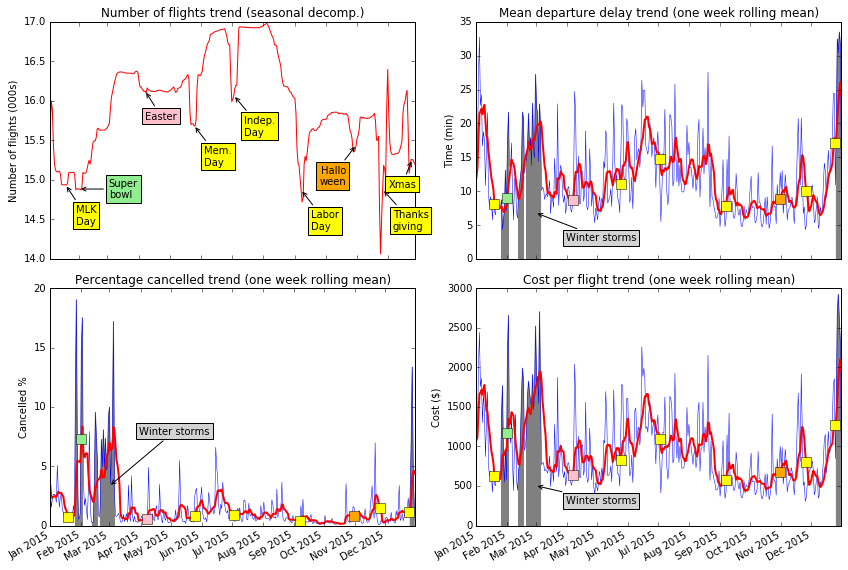
\includegraphics[width=1.1\textwidth]{../figures/exploration/delays_year.png}}
\caption{Variation in the daily delays and cancellations through 2015}
\label{delaysyear}
\end{figure}

The trends for departure delay, percentage cancelled and cost per flight through 2015 are shown in Figure \ref{delaysyear}, alongside the trend in the number of flights. These are much noisier than the number of flights, and show no significant weekly component, therefore I instead applied a one-week rolling average to obtain the trend, which is shown in red on top of the raw data in blue. The coloured squares indicate the positions of the dates that led to features in the number of flights trend, labelled in the top left panel. Of these dates only Christmas and Thanksgiving appear close to spikes in the delays and cancellations however, the other events do not have a significant effect. There is still a slight increase, in delays at least, over summer, however the raw data is swamped by large spikes throughout the year. The largest of these in the delay and especially the cancellations appear in the winter, from January to March and at the end of December. I already postulated in the previous section that many delays and cancellations, at least in the North East, are due to winter storms, and so I have filled in in grey on the three plots the date ranges over which large winter storms hit the USA (with my definition of large being having it's own Wikipedia article).\footnotemark[8]\footnotetext[8]{\url{https://en.wikipedia.org/wiki/January_2015_North_American_blizzard}}\footnotemark[9]\footnotetext[9]{\url{https://en.wikipedia.org/wiki/January_31_\%E2\%80\%93_February_2,_2015_North_American_blizzard}}\footnotemark[10]\footnotetext[10]{\url{https://en.wikipedia.org/wiki/Early_March_2015_United_States_winter_storm}}\footnotemark[11]\footnotetext[11]{\url{https://en.wikipedia.org/wiki/Late_December_2015_North_American_storm_complex}} These winter storms line up well with the spikes in cancellation, as well as prolonged periods of delays, and therefore seem to be one of the most influential features in their occurrence.

To probe further the effect of weather on delays, I looked at how the different components of delay varied over the year (again taking a one-week rolling average), rather than just the total. In the dataset the  delays are split into components due to one of five causes:\footnotemark[12]\footnotetext[12]{\url{http://www.rita.dot.gov/bts/help/aviation/html/understanding.html}} `Carrier', due to circumstances within the airlines control (e.g. crew problems); `Weather', significant meteorological events (e.g. blizzards); `NAS', due to the National Aviation System (e.g. air traffic control); `Late Aircraft', self-explanatory; `Security', due to security problems (e.g. evacuations).  Na\"{i}evly one may expect the `Weather' component to contain the delay due to weather, however non-extreme weather is assigned to the National Aviation System component `NAS', and delays due to weather will have a knock-on effect at other airports due to `Late Aircraft'. Figure \ref{delaytypesyear} shows the contributions to the total delay of these five components across the year for the states of New York, Colorado, Florida and Hawaii. First apparent is that the biggest contribution to delays is late aircraft, with that assigned to `Weather' -- that is, extreme weather -- only small. However `NAS' also tends to increase in size with weather, and I imagine this is down to the non-extreme weather assigned to it. Aside from these, `Carrier' is near constant throughout the year while `Security' is negligible.

\begin{figure}[h]
\centering
\hbox{\hspace{-0.5in}
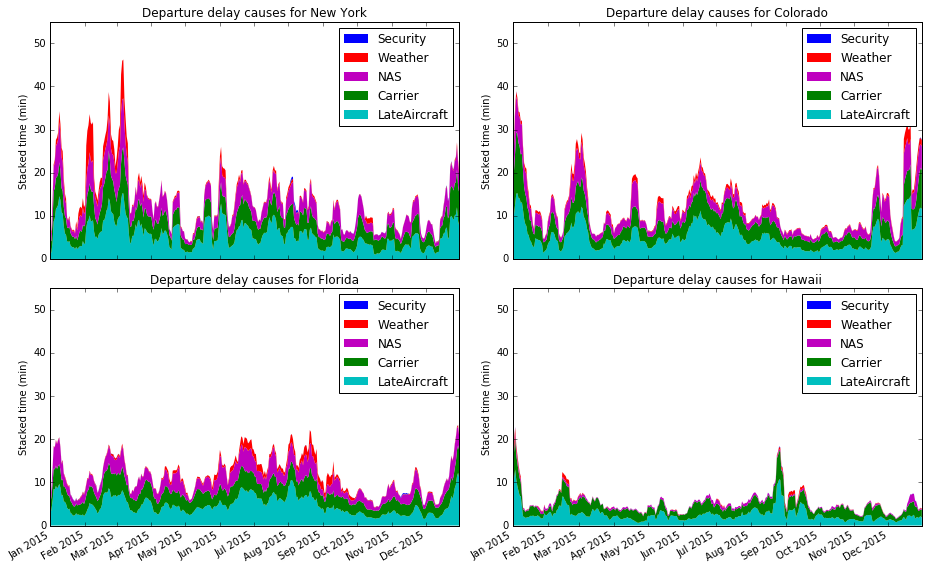
\includegraphics[width=1.1\textwidth]{../figures/exploration/delaytypes_year.png}}
\caption{Contributions to the total delay by airline, and daily variation through 2015 for New York, Florida and Hawaii}
\label{delaytypesyear}
\end{figure}

Looking at the effect of extreme weather on delays, the early year winter storms were most keenly felt in New York, which shows three clear peaks in January and February. However the effect of these storms is felt thoughout the county thanks to late aircraft, with belated peaks seen in delays as far as Hawaii. Colorado was hit harder by the winter storm at the end of the year, and also has smaller peaks in extreme weather delays thanks to local snowstorms in April\footnotemark[13]\footnotetext[13]{\url{http://www.foxnews.com/us/2016/04/16/snow-storm-forces-cancellation-almost-700-flights-at-denver-airport.html}} and May\footnotemark[14]\footnotetext[14]{\url{https://weather.com/storms/winter/news/winter-storm-venus-snow-mothers-day-weekend}}. In contrast, Florida is quiet throughout winter, and instead has its largest delays in summer, with extreme weather delays throughout hurricane season of July to October; Hawaii sees little delays from weather at all, and as a result has low delays throughout the year. It is clear therefore that weather is one of the main contributing factors to delays and cancellations, causing much of the variation seen both across the country and through the year.

\section*{Predicting cancellations}

\subsection*{Building features from the original dataset}

The airline industry has very tight margins, with a typical profit of $~$\$5.50 per passenger;\footnotemark[15]\footnotetext[15]{\url{http://edition.cnn.com/2014/06/03/travel/how-airlines-make-less-than-6/}} assuming an average plane has 150 seats, this corresponds to a profit of just \$825 per flight. Therefore cancellations are very costly to the business: assuming the loss of \$8,000 per cancellation I've used thus far, to simply cover the cost of one cancelled flight 10 more would need to be run. Therefore if the airline could predict the flights that were highly likely to be cancelled, and not run these flights in the first place, a signficant amount of money could be saved. This is a classification problem: there is a binary variable in the data already corresponding to a cancellation, so, using the insights gained from the data exploration thus far, I built a number of features from the initial dataset to be used in predicting cancellations.

Firstly the temporal features. I found in Figure \ref{numflightsyear} that the flights show a weekly periodicity, so I represented the date of the flight with features corresponding to the {\bf day of the week} (taking a value from 0 to 6) and the {\bf week in the year} (taking a value from 0 to 52). I also created a feature for {\bf time of departure} (in minutes after midnight), which, averaged across the year, showed a slight effect on cancellations: from a minimum around 9am the percentage cancelled slowly increases until 9pm, although overnight cancellations are much more erratic. Both Christmas and Thanksgiving also led to a slight increase in the probability of cancellation, so {\bf days from Christmas} and {\bf days from Thanksgiving} were added to the model (taking values of -183 to +183 to distinguish before and after, as the number of flights behaved differently either side); other public events also affected the total number of flights, but in a similar fashion, so a similar feature was added for {\bf days from public event}, which measures the number of days to the closest of the events (excluding Thanksgiving and Christmas) indicated on Figure \ref{numflightsyear}. Finally, I found in Figure \ref{delaysyear} that, of all events, winter storms have the largest effect on cancellations, so a feature was added for {\bf days after winter storm} (taking values of 0 to +365, as the storm has little effect before it hits), albeit this requires knowing in advance when a storm is likely to hit.

Figure \ref{costairports} showed there is a definite geographical influence on cancellations, and, as shown in Figure \ref{delaytypesyear}  this is mainly due to the different weather in different regions. Therefore creating {\bf dummy variables for state} of the origin airport can encode well the variability with geography. The most frequently cancelled routes in the dataset also tend to be some of the shortest, so {\bf distance of flight} is also a useful feature. The size of the airport the flight leaves from may also affect the likelihood of cancellation, so this is added as a feature by the {\bf number of flights} out of the airport in a year. Equally how busy an airport is, compared to normal, may affect cancellations, so I added a feature for the {\bf busy-ness} of an airport: the number of departing flights on a given day divided by the mean daily number of flights across the year. Finally, Figure \ref{normalisedcostbycarrier} showed that, independent of geography, the airline running the flight also affected it's cancellation probability, so I also added {\bf dummy variables for airline}. Altogether this comes to 77 features.

\subsection*{Evaluating the models}

As the model will be performing classification, it's output will be a 0 (not cancelled) or a 1 (cancelled) for every row of features in the test set. Combining these predictions with the actual values gives the confusion matrix: the number of true negatives, false negatives, false positives and true positives. Taking (\#true positives/(\#true positives + \#false positives)) gives the {\bf precision}, the probability that a flight predicted to be cancelled is acually cancelled, and taking (\#true positives/(\#true positives + \#false negatives)) gives the {\bf recall}, the proportion of actually cancelled flights we are predicting. I also kept note of the {\bf F1 score} ($2PR/(P+R)$) and the {\bf accuracy} (\#true positives + \#true negatives)/\#test samples, however it's worth noting that as only $~$2\% of flights are cancelled, by guessing every flight as not cancelled the accuracy would already by 98\%. Finally, using the previously stated assumptions of +\$825 profit per flight and -\$8000 loss per cancellation, I also calculated the cost that would be saved by not running the flights identified as cancelled by the model: (\$8000$\times$\#true positives -\$825$\times$\#false positives). Dividing this by the number of samples in the test set -- so as to be independent of sample size -- gives the {\bf cost saved per flight}, which is probably the best measure of evaluation as it is (a rough estimate of) the savings to the business. As a reference point, predicting no cancellations would give values for these evaluation metrics of:

\noindent precision = 0; recall = 0; F1 = 0; accuracy = 0.98; cost save per flight = \$0

The entire dataset of $\sim$6 million rows is too large to train on my laptop, so I took a random sample of 20\% of the data and used the first half (so $\sim$600,000 rows) for a 10-fold cross validation of the models, keeping the second half to use as a test set. All features were scaled before training by centering on the mean and scaling to unit variance.

\subsection*{Logistic regression}

\begin{figure}[h]
\centering
\hbox{\hspace{-0.5in}
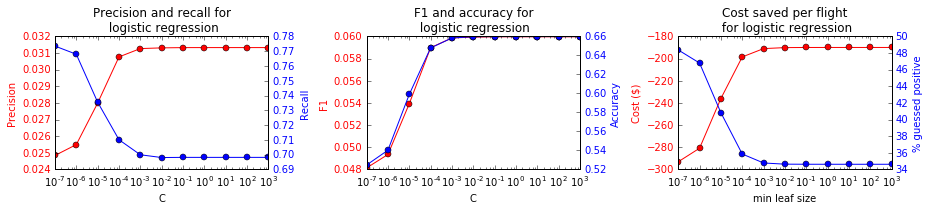
\includegraphics[width=1.15\textwidth]{../figures/classification/log_reg_C.png}}
\caption{Logistic regression on the initial dataset with varying C}
\label{logreg}
\end{figure}

To begin I trained a classifier using perhaps the simplest method -- logistic regression -- with balanced class weights to account for the small proportion of cancelled flights (without balancing no cancellations are predicted). This model was then optimised for the regularisation C: high C corresponds to overfitting the training set, low C to underfitting. Figure \ref{logreg} shows how the various evaluation metrics depend on C. For all the values the recall is high but the precision low, this is because of the large number of positive predictions, between 30-50\%, compared to just 2\% positive in the actual values. Increasing C decreases the number of positive predictions, increasing the precision and decreasing the recall, and in this region (above C=$10^{-2}$) the accuracy and cost saved per flight is highest. This doesn't mean much however: the accuracy is far worse than predicting no cancellations, and implementing the model would give a -\$190 loss per flight. Applying this model on the test set gives:

\noindent precision = 0.03; recall = 0.70; F1 = 0.06; accuracy = 0.67; cost saved per flight = -\$185.72

Nevertheless, we can still use the coefficients found by logistic regression to get some idea of the linear trend for each variable, specifically to compare performance between airlines, as is shown in Figure \ref{logregcarrier}. This in fact looks much like the previous measure of the percentage cancelled compared to the airport average, plotted back in Figure \ref{normalisedcostbycarrier} and again finds Delta to be the best performing (though by a greater degree here) and American Eagle the worst.

\begin{figure}[h]
\centering
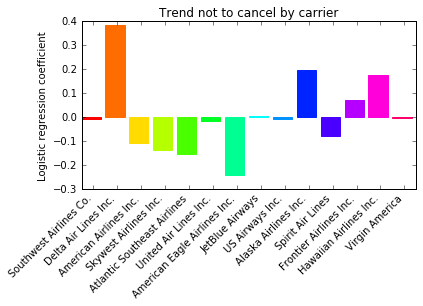
\includegraphics[width=0.55\textwidth]{../figures/classification/log_reg_carrier.png}
\caption{Logistic regression coefficients for cancellation by airline}
\label{logregcarrier}
\end{figure}

\subsection*{Random forest classifier}

\begin{figure}[h]
\centering
\hbox{\hspace{-0.5in}
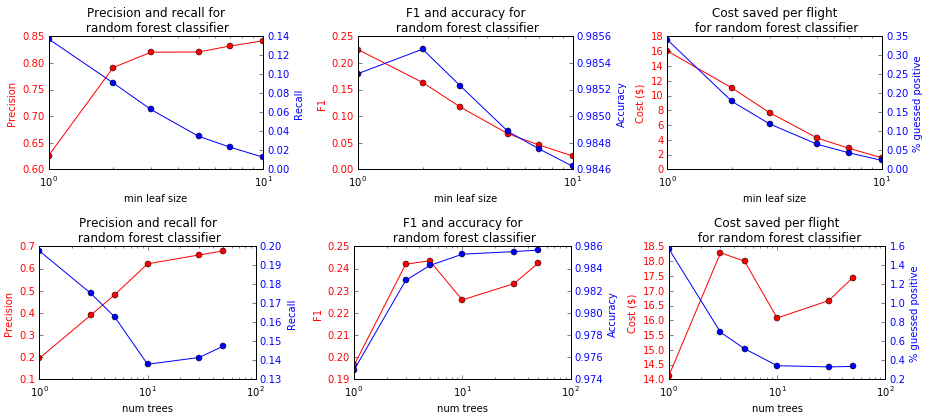
\includegraphics[width=1.15\textwidth]{../figures/classification/rf_reg_leaves.png}}
\caption{Random forest classification on the initial dataset, varying the minimum samples per leaf and number of trees}
\label{randfor}
\end{figure}

The next model I trained was a random forest classifier, which -- as it is constructed from an ensemble of decision trees -- should be able to deal better with the dummy variables and relationships between features in the dataset, while still being fast to run. This model was then optimised on the training set for the `minimum samples per leaf', that is the smallest number of samples upon which a classification decision can be based, and the number of trees from which the forest is constructed. Figure \ref{randfor} shows the effect of varying minimum leaf size for 10 trees, and the effect of varying the number of trees for 1 sample minimum per leaf.

Increasing the minimum leaf size means increasingly more similar cancellations are required to identify a cancellation in the test set, so the precision increases but the recall drops dramatically. This results in a comparable decrease in the cost: a minimum of one sample per leaf performs best. Increasing the number of trees improves the accuracy of the model and the precision, but in decreasing the variance of the model (by less over-fitting) it also significantly decreases the recall, at least for ensembles of 10 trees or fewer. Above 10 trees the model improves by all measures the larger the forest gets, and so the highest cost saved per flight will be with the largest forest. However, in the range of 1-50 trees the model was tested over, the highest cost occurs at the point at which the precision and recall cross over -- an ensemble of 3 trees -- rather than for the larger forest when both are increasing. Applying this classifier to the test set, with 3 trees and a minimum leaf size of 1, gives:

\noindent precision = 0.380; recall = 0.170; F1 = 0.234; accuracy = 0.983; cost saved per flight = +\$17.05

\noindent So by all measures except recall (as we are predicting considerably fewer cancellations) the model performs better than logistic regression; indeed by implementing this random forest a non-negligible cost could be saved per flight.

\subsection*{Adding features to the dataset}

Given that I now had a model that was performing well at predicting cancellations with the current features, all built from the initial dataset, my next step was to try to improve the cost saved by introducing new features from external data sets. For every flight in the original database the city of the origin airport is also specified, and so this is straightforward to combine with urban area data collected by the United States Census Bureau. From the 2010 census they have a database\footnotemark[16]\footnotetext[16]{\url{https://www.census.gov/geo/reference/ua/urban-rural-2010.html}} of various measures of population and land type for all urban areas in the USA. Once the data is cleaned and merged, 87\% of the airports can now be associated with urban area data. From this dataset I constructed two features. The {\bf population density} acts as a measure of how urban the surrounding area of the airport is, with factors such as pollution or congestion potentially leading to cancellations. The {\bf fraction of the surrounding area that is water} indicates how close an airport is to seas or lakes, and so the potential risk from flooding or more extreme weather. For those airports without urban area data, I set their values for the two features to be the mean of those in their state. Adding these features to the random forest clasiifier and applying it to the test set gives:

\noindent precision = 0.388; recall = 0.172; F1 = 0.238; accuracy = 0.983; cost saved per flight = +\$17.41

\noindent so these two features both slightly increase the precision and recall, and hence the cost saved.

From the exploration of the initial dataset, it was clear that weather was incredibly important for determining cancellations. Therefore, adding a weather forecast for each airport on each day should make a big improvement to the predictive capabilities of the model. Luckily the website Weather Underground\footnotemark[17]\footnotetext[17]{\url{https://www.wunderground.com/history/airport}} has historical weather data for the USA, searchable in a specified time frame by airport code, and stored in .csv format. By scraping this site I was able to get weather data for every airport for every day of 2015. The numerical fields I added to the model where the mean daily {\bf temperature}, {\bf dew point}, {\bf sea level pressure}, {\bf visibility} and {\bf wind speed}, the {\bf total precipitation} and the {\bf cloud cover}. Additionally there was a text column that listed any extreme weather types observed on the day. By cleaning and separating the different types, I was also able to create dummy variables for {\bf fog}, {\bf hail}, {\bf rain}, {\bf snow}, {\bf thunderstorm} and {\bf tornado}. Adding these to the classifier leads to a bigger increase in the cost saved:

\noindent precision = 0.376; recall = 0.180; F1 = 0.244; accuracy = 0.983; cost saved per flight = +\$18.06

Finally, the initial dataset also has the tail number of the plane for each flight. As the most frequently cancelled flights tend to be the shortest, there may also be some dependence on the type of plane: smaller, local flights will be cheaper to cancel than long distance flights with lots of passengers. Equally some planes may be more prone to mechanical problems than others, and this too could lead to more cancellations. A database of plane details, including tail number, for domestic US aircraft can be found online in many places, so, for ease I used a copy already in .csv format.\footnotemark[18]\footnotetext[18]{\url{http://euler.stat.yale.edu/~tba3/class_data/plane-data.csv}} Merging with initial database gives plane details for 62\% of the flights. For each plane the model, manufacturer, aircraft type and engine type is specified; due to the large number of models -- and the likelihood that specifying a manufacturer, aircraft type and engine type would be equivalent to naming a certain model -- I created {\bf dummy variables for  manufacturer}, {\bf aircraft type} and {\bf engine type}. There was also a numerical field for the {\bf age of aircraft} which I added as a feature, assuming the mean value for those which had no data. Added to the classifier these features gives:

\noindent precision = 0.395; recall = 0.173; F1 = 0.240; accuracy = 0.983; cost saved per flight = +\$17.59

\noindent so the precision has increased, but to the detriment of the recall, and as a result the cost saved decreases.

\begin{figure}[h]
\centering
\hbox{\hspace{-0.5in}
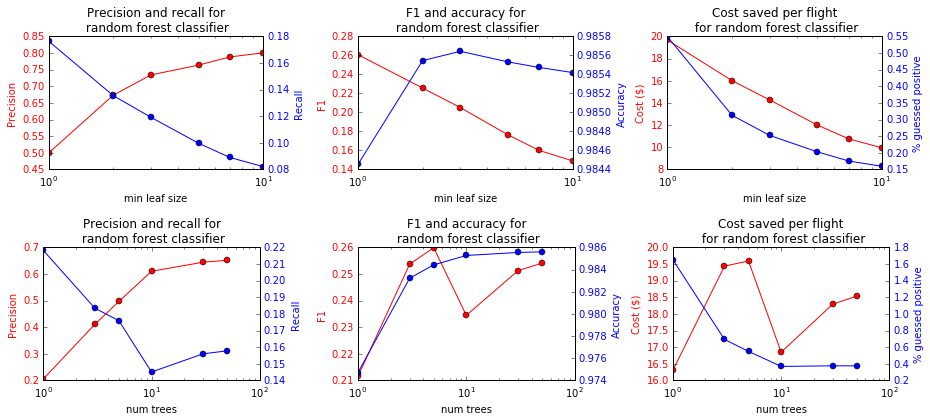
\includegraphics[width=1.15\textwidth]{../figures/classification/rf2_reg_leaves.png}}
\caption{Random forest classification on the dataset with external features added, varying the minimum samples per leaf and number of trees}
\label{randfor2}
\end{figure}

However, before passing judgement on the usefulness of the new features, I first re-optimised the random forest classifier with all features included (the 77 original plus 46 new, giving 123 in total). Figure \ref{randfor2} shows the effect of varying minimum leaf size for 3 trees, and the effect of varying the number of trees for 1 sample minimum per leaf, the evaluation metrics behave similarly to before. The best cost saving now occurs for an ensemble of 5 trees rather than 3, and performs best with the urban area and weather features included, but not the aircraft details. However instead optimising for accuracy, the model gets the most predictions right by including the aircraft details, with minimum three samples per leaf and a forest of 50 trees. The cost-optimised model gives the best cost saving on the test set:

\noindent precision = 0.451; recall = 0.174; F1 = 0.251; accuracy = 0.984; cost saved per flight = +\$18.44

\noindent while the accuracy-optimised model gets the most predictions correct, with a high precision:

\noindent precision = 0.793; recall = 0.103; F1 = 0.182; accuracy = 0.986; cost saved per flight = +\$12.13

However, both these models require accurate knowledge of the weather, which, for predicting cancellations some distance into the future, may not be feasible. Therefore, for a final test of applicability, I ran the cost-optimised model on the test set without meteorological features, that is without the daily weather predictions by airport and also the dates of winter storms. This gives:

\noindent precision = 0.496; recall = 0.145; F1 = 0.224; accuracy = 0.985; cost saved per flight = +\$15.65

\noindent so a (smaller) cost saving is still possible. This is still biased, however, by the fact that the train and test flights are taken from the same year: a storm on a certain day at a certain airport will affect all flights leaving on that day in 2015, but not those leaving on that day in 2016; therefore a combination of the state and time variables act as a conduit for the weather.

Given longer than a week, I would therefore train a model -- using the random forest classifier above -- across multiple years, so that it learns seasonal trends in weather rather than discrete events. This should then be tested on data from a later year, not in the training set, to gain a true measure of the applicablity of this model for predicting future cancellations. The biggest increase in performance will likely come, not with new features or better algorithms, but with increasing the size of the training set: as cancellations are a rare event and only 10\% of the total data was used to train the above classifiers -- a result of my limits in both time and computing capacity -- increasing this fraction should lead to big increases in both precision and recall, and hence the costs saved. Additionally the features I've built will also be relevant for predicting delays, and so could be used as the basis for a regressor predicting delay times, and hence -- especially by predicting `carrier' delays, the delays due to the airlines operations -- where the airlines should focus more of their resources to keep overall delays down. Nevertheless, for flights in 2015 my random forest classifier is able to identify savings of approximately {\bf \$18 per flight} -- a {\bf 2.2\% increase in the profit} -- totalling, across all airlines, to {\bf more than \$10 million saved a year}.

\subsection*{Summary}

In this assignment I've looked at delays and cancellations of US domestic flights across 2015, determining which airlines, regions and times of year perform best and worst, and building a classifier to predict cancellations. Among the larger airlines, those running a hub-and-spoke network perform better than average on delays and cancellations, while those running a point-to-point network perform worse. For smaller airlines, those running regional networks -- particularly in region of the USA that have less extreme weather -- have the lowest average delay times and number of cancellations, while those running nation-wide networks have the highest. The most cancellations occur in the winter months, and these are mainly due to snow storms, with the North Eastern USA most affected. Delays are more evenly spread throughout the year, but there is a clear seasonal trend on a state-by-state level: those in the North East have the longest delays over winter, as a result of snow; those in the South East have the longest delays over summer, as a result of tropical storms. Although weather is the most important cause of delays and cancellations, both Thanksgiving and Christmas also lead to a nation-wide increase.

Using these insights, I built a classifier for predicting cancelled flights. Adding features from the dataset encoding the airline, geographical and temporal behaviour, and encorporating external datasets to build features describing the area surrounding the departure airport, the daily weather at each airport and the type of aircraft, an optimised random forest classifier was able to predict cancellations with 0.45 precision and 0.17 recall, leading to an approximate saving of \$18 per flight, or \$10 million across the year.

\end{document}